\documentclass[12pt]{article}
\usepackage[utf8]{inputenc}
\usepackage[pdftex]{graphicx}
\usepackage{graphicx}
\usepackage{geometry}
\usepackage{indentfirst}
\usepackage{setspace}
\usepackage{anysize}
\usepackage{makeidx}
\usepackage[brazil]{babel}
\usepackage{longtable}
\usepackage{multirow} 
\usepackage{hyperref}
\usepackage{subfig}
\makeindex

\newcommand{\longtableendfoot}{Continuará na próxima página}

\geometry{
	verbose,
	a4paper,
	left = 30mm,
	top = 30mm,
	right = 20mm,
	bottom = 20mm
}

\begin{document}

\begin{figure}
    \centering
    
\includegraphics[width=16cm]{fga.jpg}
\end{figure}

\begin{titlepage}
% \doublespacing
\centering

\normalfont


\vspace{0.1\textheight}
\vbox{\normalfont{UNB - UNIVERSIDADE DE BRASÍLIA\\CAMPUS GAMA}}
\large{Universidade de Brasília - UnB Gama\\}
\vspace{3cm}


\vbox{\Huge
%Nome do Trabalho
GamePlay

%\ver

\vspace{0.03\textheight}
\hrule }

\vbox{
%Nome da Matéria
Introdução à Computação Gráfica
}
\vspace{0.2\textheight}
%Nomes
\vbox{\scshape
{}
  Developers: Elmar Roberto, Daniel Moura e Eduardo Gomes
  }
\vspace{0.2cm}
{}
\centering
elmarunb@gmail.com | danmoura17@gmail.com | eduardoqgomes@gmail.com \\
\vspace{0.2\textheight}
Brasília, DF~-~\the\year
\end{titlepage}

\onehalfspacing
\tableofcontents
\newpage

\part{Escopo Geral}

Dando início ao jogo a partir do menu principal, a corrida se inicia. O jogador deve apenas movimentar o carro com as setas do teclado ou com as teclas 'w','a','s' e 'd', onde cada função esta detalhada na imagem abaixo. A utilização do mouse é apenas para movimentar a câmera. O jogador deve seguir o trajeto da pista coletando os nitros para repor gasolina e coletando os objetos para ganhar pontos. Evitando sair da pista e não deixando acabar a gasolina, o carro chegará facilmente a linha de chegada encerrando o jogo. \\\\ 

\begin{figure}[!h]
	\centering
		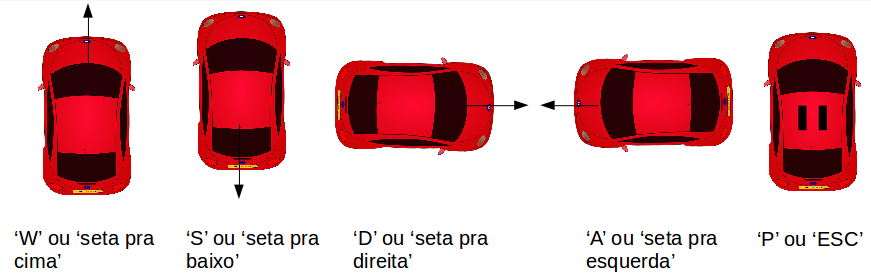
\includegraphics[scale=0.5]{movimentos}
\end{figure}

\begin{figure}[!h]
	\centering
		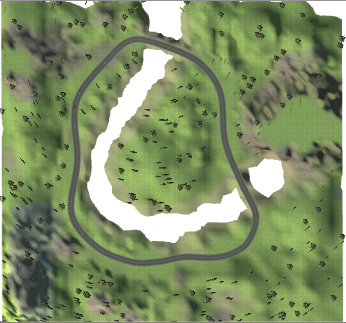
\includegraphics[scale=0.8]{percurso}
	\caption{Mapa completo do jogo}
\end{figure}

\end{document}